
\subsection{研究目标}
% 武旭同话术,待修改
基于上述研究进展,本研究面向社会-水文学研究前沿和黄河流域高质量发展的国家需求,以黄河流域为研究区,结合水文气象观测、社会经济统计、历史数据重建、遥感反演等获取多源数据,借助统计分析和模型模拟等手段,分析黄河流域人水关系的演变过程和驱动机制。具体研究目标如下:

(1)定义便于研究的“流域人水关系”,发展识别其演变规律的分析框架,分别在历史时期和现代治黄时期,定量划分黄河流域人水关系演变的主要阶段与过程。
(2)发展流域人水关系演变机制分析的因果推断方法,建立黄河流域社会-生态系统的多主体模型,识别推动人水关系变化的关键机制,定量评估其产生的影响。


\subsection{研究内容}

针对流域这个特定的人地关系地域系统(或社会-生态系统)给出“人水关系”的概念定义,为满足不同时间尺度的分析需要,建立流域系统层面的人水关系变化分析框架。在此框架的基础上,本研究具体包含以下主要内容:

% 开题报告
(1)黄河流域历史时期流域水沙特征演变:识别历史时期不断增强的人类活动压力超越气候周期变化的驱动力的时间,以及两者主导并推动黄河流域水沙特征突破临界点的稳态转换过程,分析该稳态转换发生之前黄河的人水关系状态。
% 接下来利用建立的分析框架对黄河流域历史上的大事记进行分析,梳理出黄河流域人-水关系演变的主要脉络。最后利用系统回顾法,整合近代有研究以来对黄河人-水关系变化的定量分析成果,建立黄河流域人-水关系变化数据库,综合分析有研究以来人-水系统的主要驱动因素及演化路径。 

(2)现代治黄时期黄河流域的水治理演变:分析上世纪六十年代有实测数据以来,黄河流域“有多少水、怎么用水、怎么分水”如何随时间变化,以及三者如何共同体现流域水治理变化,并解释这些变化背后流域系统如何被人类活动所主导。

(3)黄河流域分水制度改革的影响:识别黄河流域在上世纪八十年代治理转变期间,先后于1987年和1998年两次改革流域水资源分配制度对流域系统的作用机制,分析其如何自上而下重塑社会-生态系统结构、以及对不同地区用水量的影响。

(4)黄河灌溉水分配的多主体建模:识别黄河流域在上世纪八十年代治理转变期间,流域用水的利益相关者对系统环境和制度变化的响应机制,分析其如何通过挑战水资源分配,自下而上地对流域转型做出适应,以及对水资源利用方式的影响。

基于上述研究内容,本研究的技术路线如图\ref{ch1:fig:workflow}所示:

\begin{figure}[htb] % use float package if you want it here
    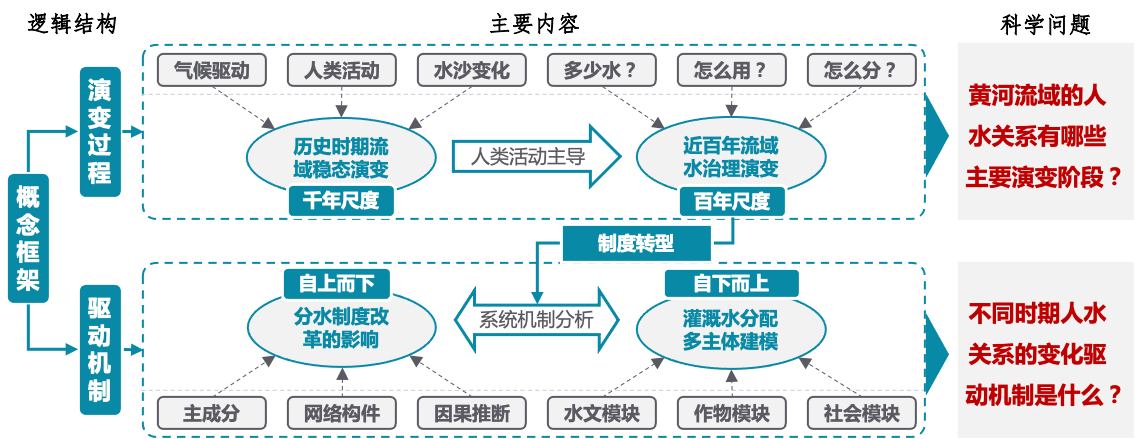
\includegraphics[width=\textwidth]{img/ch1/ch1_workflow.png}
    \caption{研究技术路线图}\label{ch1:fig:workflow}
\end{figure}

首先,发展流域系统人水关系演变的概念框架,明晰流域人水关系的概念内涵,厘定怎样的变化可以被识别为发生了“流域人水关系演变”,以及有哪些潜在的驱动机制会导致这些变化。接下来利用研究概念框架,分别在历史时期和现代治黄时期识别流域人水关系的演变过程:
(1)人类主导流域水沙特征变化是黄河人水关系变化的关键标志,黄河流域的水沙特征在历史时期发生从气候周期驱动向人类活动主导的过程,需要识别这一稳态转换的发生过程。
(2)水治理是现代流域人水关系变化的主要驱动力,黄河流域的“自然-社会二元水循环”在现代治黄时期则已由人类活动主导,需要识别流域水治理系统发生稳态转换的过程。
通过整合历史时期和人民治黄时期的人水关系演变,可以回答“黄河流域的人水关系有哪些主要演变阶段?”的科学问题,并总结各阶段黄河流域人水关系的演变特征。

针对现代治黄时期流域治理转变由人类制度主导的特点,接下来的两章以制度变化为落脚点,以对黄河流域影响最为深远的水资源分配制度为例,分别从自上而下和自下而上两个路径分析流域人水关系变化的驱动机制:
(1)自上而下:使用主成分分析、社会-生态系统网络构件识别、因果推断模型,分析制度改革对黄河流域系统结构及不同地区用水量的影响。
(2)自下而上:使用由人类模块和自然模块耦合构成的多主体模型,分析农业用水决策者的如何响应环境和制度变化,改变其水资源利用的过程。

\subsection{关键科学问题}

(1)黄河流域的人水关系有哪些主要演变阶段?

(2)不同时期人水关系变化的驱动机制是什么?
